\documentclass{article}
\pdfminorversion=6
\usepackage[utf8]{inputenc}
\usepackage{amssymb, amsmath, amsthm}
\usepackage{thmtools, mathtools, mathrsfs}
\usepackage{amsfonts}
\usepackage{forloop}
\usepackage{stmaryrd}
\usepackage[sort&compress,numbers]{natbib}
\usepackage{subcaption}
\usepackage{graphicx}
\usepackage{caption}
\usepackage{float}
\usepackage{bm}
\usepackage{tikz}
\usepackage{tikz-cd}

\newcommand{\defvec}[1]{\expandafter\newcommand\csname v#1\endcsname{{\mathbf{#1}}}}
\newcounter{ct}
\forLoop{1}{26}{ct}{
    \edef\letter{\alph{ct}}
    \expandafter\defvec\letter
}

% captial \vA
\forLoop{1}{26}{ct}{
    \edef\letter{\Alph{ct}}
    \expandafter\defvec\letter
}

\newcommand{\dm}[1]{\ensuremath{\mathrm{d}{#1}}} % dx dy dz dmu
\newcommand{\RN}[2]{\frac{\dm{#1}}{\dm{#2}}} % (Radon-Nikodym) derivative
\newcommand{\PD}[2]{\frac{\partial #1}{\partial #2}} % partial derivative
\newcommand{\overbar}[1]{\mkern 1.5mu\overline{\mkern-1.5mu#1\mkern-1.5mu}\mkern 1.5mu}
\newcommand{\win}{\vW_{\text{in}}}
\newcommand{\wout}{\vW_{\text{out}}}
\newcommand{\bout}{\vb_{\text{out}}}
\newcommand{\reals}{\mathbb{R}}

\newcommand{\manifold}{\mathcal{M}}

\DeclareMathOperator{\relu}{ReLU}

% if you need to pass options to natbib, use, e.g.:
%     \PassOptionsToPackage{numbers, compress}{natbib}
% before loading neurips_2023

% ready for submission
% \usepackage{neurips_2023}

% to compile a preprint version, e.g., for submission to arXiv, add the
% [preprint] option:
%     \usepackage[preprint]{neurips_2023}

% to compile a camera-ready version, add the [final] option, e.g.:
%     \usepackage[final]{neurips_2023}

% to avoid loading the natbib package, add option nonatbib:
     \usepackage[]{neurips_2023}
     
\usepackage[utf8]{inputenc} % allow utf-8 input
\usepackage[T1]{fontenc}    % use 8-bit T1 fonts
\usepackage{hyperref}       % hyperlinks
\usepackage{url}            % simple URL typesetting
\usepackage{booktabs}       % professional-quality tables
\usepackage{amsfonts}       % blackboard math symbols
\usepackage{nicefrac}       % compact symbols for 1/2, etc.
\usepackage{microtype}      % microtypography

\newcommand{\probP}{\text{I\kern-0.15em P}}

\newtheorem{theorem}{Theorem}
\newtheorem{prop}{Proposition}
\theoremstyle{definition}
\newtheorem{definition}{Definition}
\theoremstyle{remark}
\newtheorem{remark}{Remark}

%\title{All line attractors are unstable, but some are more unstable than others}
%\title{Stable and unstable gradients near identical recurrent computation}
%\title{Stable and unstable gradients near identical recurrent computation}
\title{RNNs with gracefully degrading continuous attractors}
%Persistent attractors 
%	Keeping explosions at bay in CANNs
%CANNs without exploding gradients? Yes we can!

% The \author macro works with any number of authors. There are two commands
% used to separate the names and addresses of multiple authors: \And and \AND.
%
% Using \And between authors leaves it to LaTeX to determine where to break the
% lines. Using \AND forces a line break at that point. So, if LaTeX puts 3 of 4
% authors names on the first line, and the last on the second line, try using
% \AND instead of \And before the third author name.

\author{%
  \'Abel.~S\'agodi %\thanks{Use footnote for providing further information about author (webpage, alternative address).} \\
 Champalimaud Centre for the Unknown\\
  \\
  Avenida da Brasília \\
  \texttt{abel.sagodi@research.fchampalimaud.org} \\
  % examples of more authors
   \And
   Piotr Sok\'\l \\
   Stony Brook University \\
   100 Nicolls Rd, Stony Brook, NY 11794, USA \\
   \texttt{piotr.sokol@stonybrook.edu} \\
   \AND
   Il Memming Park \\
   Champalimaud Centre for the Unknown \\
   Avenida da Brasília  \\
   \texttt{memming.park@research.fchampalimaud.org} 
}

\begin{document}

%keywords: 
%neural computation, robustness, bifurcation analysis, exploding gradient problem, continuous attractors, persistence of invariant manifolds 
    
%TLDR


\maketitle

\begin{abstract}
Attractor networks are essential theoretical components in recurrent networks for memory, learning, and computation.
However, the continuous attractors that are essential for continuous-valued memory suffer from structural instability---infinitesimal changes in parameter can destroy the continuous attractor.
Moreover, the perturbed system can exhibit divergent behavior with associated exploding gradients.
This poses a question about the utility of continuous attractors for systems that learn using gradient signals.
%This poses a problem in biological neural networks, as they are constantly subjected to perturbations caused by noise. Certain systems (e.g. systems with an unbounded attractor) can be perturbed in such a way, that not only do they bifurcate, but start exhibitung divergent behavior, which is especially problematic for systems that are learning (for example under gradient descent).
To address this issue, we use Fenichel's persistence theorem from dynamical systems theory to show that bounded attractors are stable in the sense that all perturbations maintain the stability.
This ensures that if there is a restorative learning signal, there will be no exploding gradients for any length of time for backpropagation.
In contrast, unbounded attractors may devolve into divergent systems under certain perturbations, leading to exploding gradients.
This insight also suggests that there can exist homeostatic mechanisms for certain implementations of continuous attractors that maintain the structure of the attractor sufficiently for the neural computation it is used in.
Finally, we verify in a simple continuous attractor that all perturbations preserve the invariant manifold and demonstrate the principle numerically in ring attractor systems.
\end{abstract}


%\section{Submission of papers to NeurIPS 2023}
%
%Please read the instructions below carefully and follow them faithfully. \textbf{Important:} This year the checklist will be submitted separately from the main paper in OpenReview, please review it well ahead of the submission deadline: \url{https://neurips.cc/public/guides/PaperChecklist}.


\section{Introduction}
%NeurIPS requires electronic submissions.  The electronic submission site is
%\begin{center}
%  \url{https://cmt3.research.microsoft.com/NeurIPS2020/}
%\end{center}

Recurrent neural/neuronal networks (RNNs) can process sequential observations and model temporal dependencies of arbitrary length.
At the same time, they are fundamentally limited by their finite-sized hidden states which form the only channel between the past and the future.
To store information over a long period of time, as many difficult tasks demand, RNNs can learn or be designed to have ``persistent memory''.
When the information of interest is continuous-valued, a natural solution is to use continuous attractors.
Continuous attractors are prevalent in theoretical neuroscience as tools to model neural representation and computation ranging from internal representations of head directions and eye positions to perceptual decision-making and working memory~\cite{Khona2022}.
Continuous attractors are also at the core of long short-term memory (LSTM)~\cite{Greff2017} units and the neural Turning machine (NTM)~\cite{Graves2014} to provide digital computer memory like properties not natural to recurrent networks. % with many applications such as meta-learning~\cite{Santoro2016}.
In fact, the critical weakness of continuous attractors is their inherent brittleness as they are rare in the parameter space, i.e., infinitesimal changes in parameters destroys the continuous attractor structures implemented in RNNs~\cite{seung1996,Renart2003}.
However, not all RNN implementations of continuous attractors behave similarly in their brittleness.

We found that in the space of RNNs, some have neighbourhoods with highly undesirable exploding gradients. We will describe some continuous attractors which have such neighbourhoods.
Consider an RNN (without input or output for now) expressed in continuous time as an ordinary differential equation:
\begin{align}\label{eq:TLN}
    \dot{\vx} = -\vx + \left[ \vW \vx + \vb \right]_{+}
\end{align}
where $\vx \in \reals^d$ is the hidden state of the network, $\vb > 0$ is the bias, and $[\cdot]_{+} = \max(0,\cdot)$ is the threshold nonlinearity per unit.
In discrete time, this corresponds to a ReLU RNN (see Sec.~\ref{sec:rnn:integration}).
The non-trivial activity of this network is limited to the (non-negative) first quadrant, outside of which the hidden state decays to the origin.

When $d=2$, we can build two kinds of continuous attractors.
First, through positive feedback, $\vW = [0, 1; 1, 0]$ and no bias $\vb = \mathbf{0}$, we can create a continuous attractor, i.e., $\dot{\vx} = 0$ on the $x_1 = x_2 \geq 0$ half-line, and surrounding attractive flow (Fig.~\ref{fig:ublabla}A left).
We refer to it as an \textbf{unbounded line attractor (UBLA)}.
For any point on the line attractor, linearization results in eigenvalues $0$ and $-2$, corresponding to the zero flow and attractive flow respectively.
When $\vW$ is perturbed, the null eigenvalue can easily become non-zero and the continuous line attractor disappears.
If it becomes negative, the system bifurcates to a stable fixed point at the origin (Fig.~\ref{fig:ublabla}A bottom).
However, if it becomes positive (Fig.~\ref{fig:ublabla}A top), \emph{the resulting flow diverges to infinity along the diagonal}.
Corresponding to the divergent flow, the backpropagating gradient over time exponentially grows in magnitude, thus rendering gradient descent impractical without truncation in time.

The second kind of continuous attractor is created through negative feedback.
By choosing $\vW = [0, -1; -1, 0]$ and $\vb = [1; 1]$, we get $\dot{\vx} = 0$ on the $x_1 = -x_2 + 1$ line segment in the first quadrant as the continuous attractor.
We refer to it as the \textbf{bounded line attractor (BLA)}.
Again, linearization on the attractor shows two eigenvalues, $0$ and $-2$, and perturbations again cause the null eigenvalue to be non-zero and the line attractor disappears.
However, surprisingly, the bifurcations are  qualitatively different.
It either bifurcates into a single stable fixed point (Fig.~\ref{fig:ublabla}B top) or two stable fixed points separated with a saddle node in between (Fig.~\ref{fig:ublabla}B bottom).
Neither of these two cases show a divergent flow, but rather consists of one or two basins of attraction.
It implies only vanishing gradients for this system and \textbf{exploding gradients will not be present for an arbitrarily long time}.

\begin{figure}[tbhp]
  \centering
  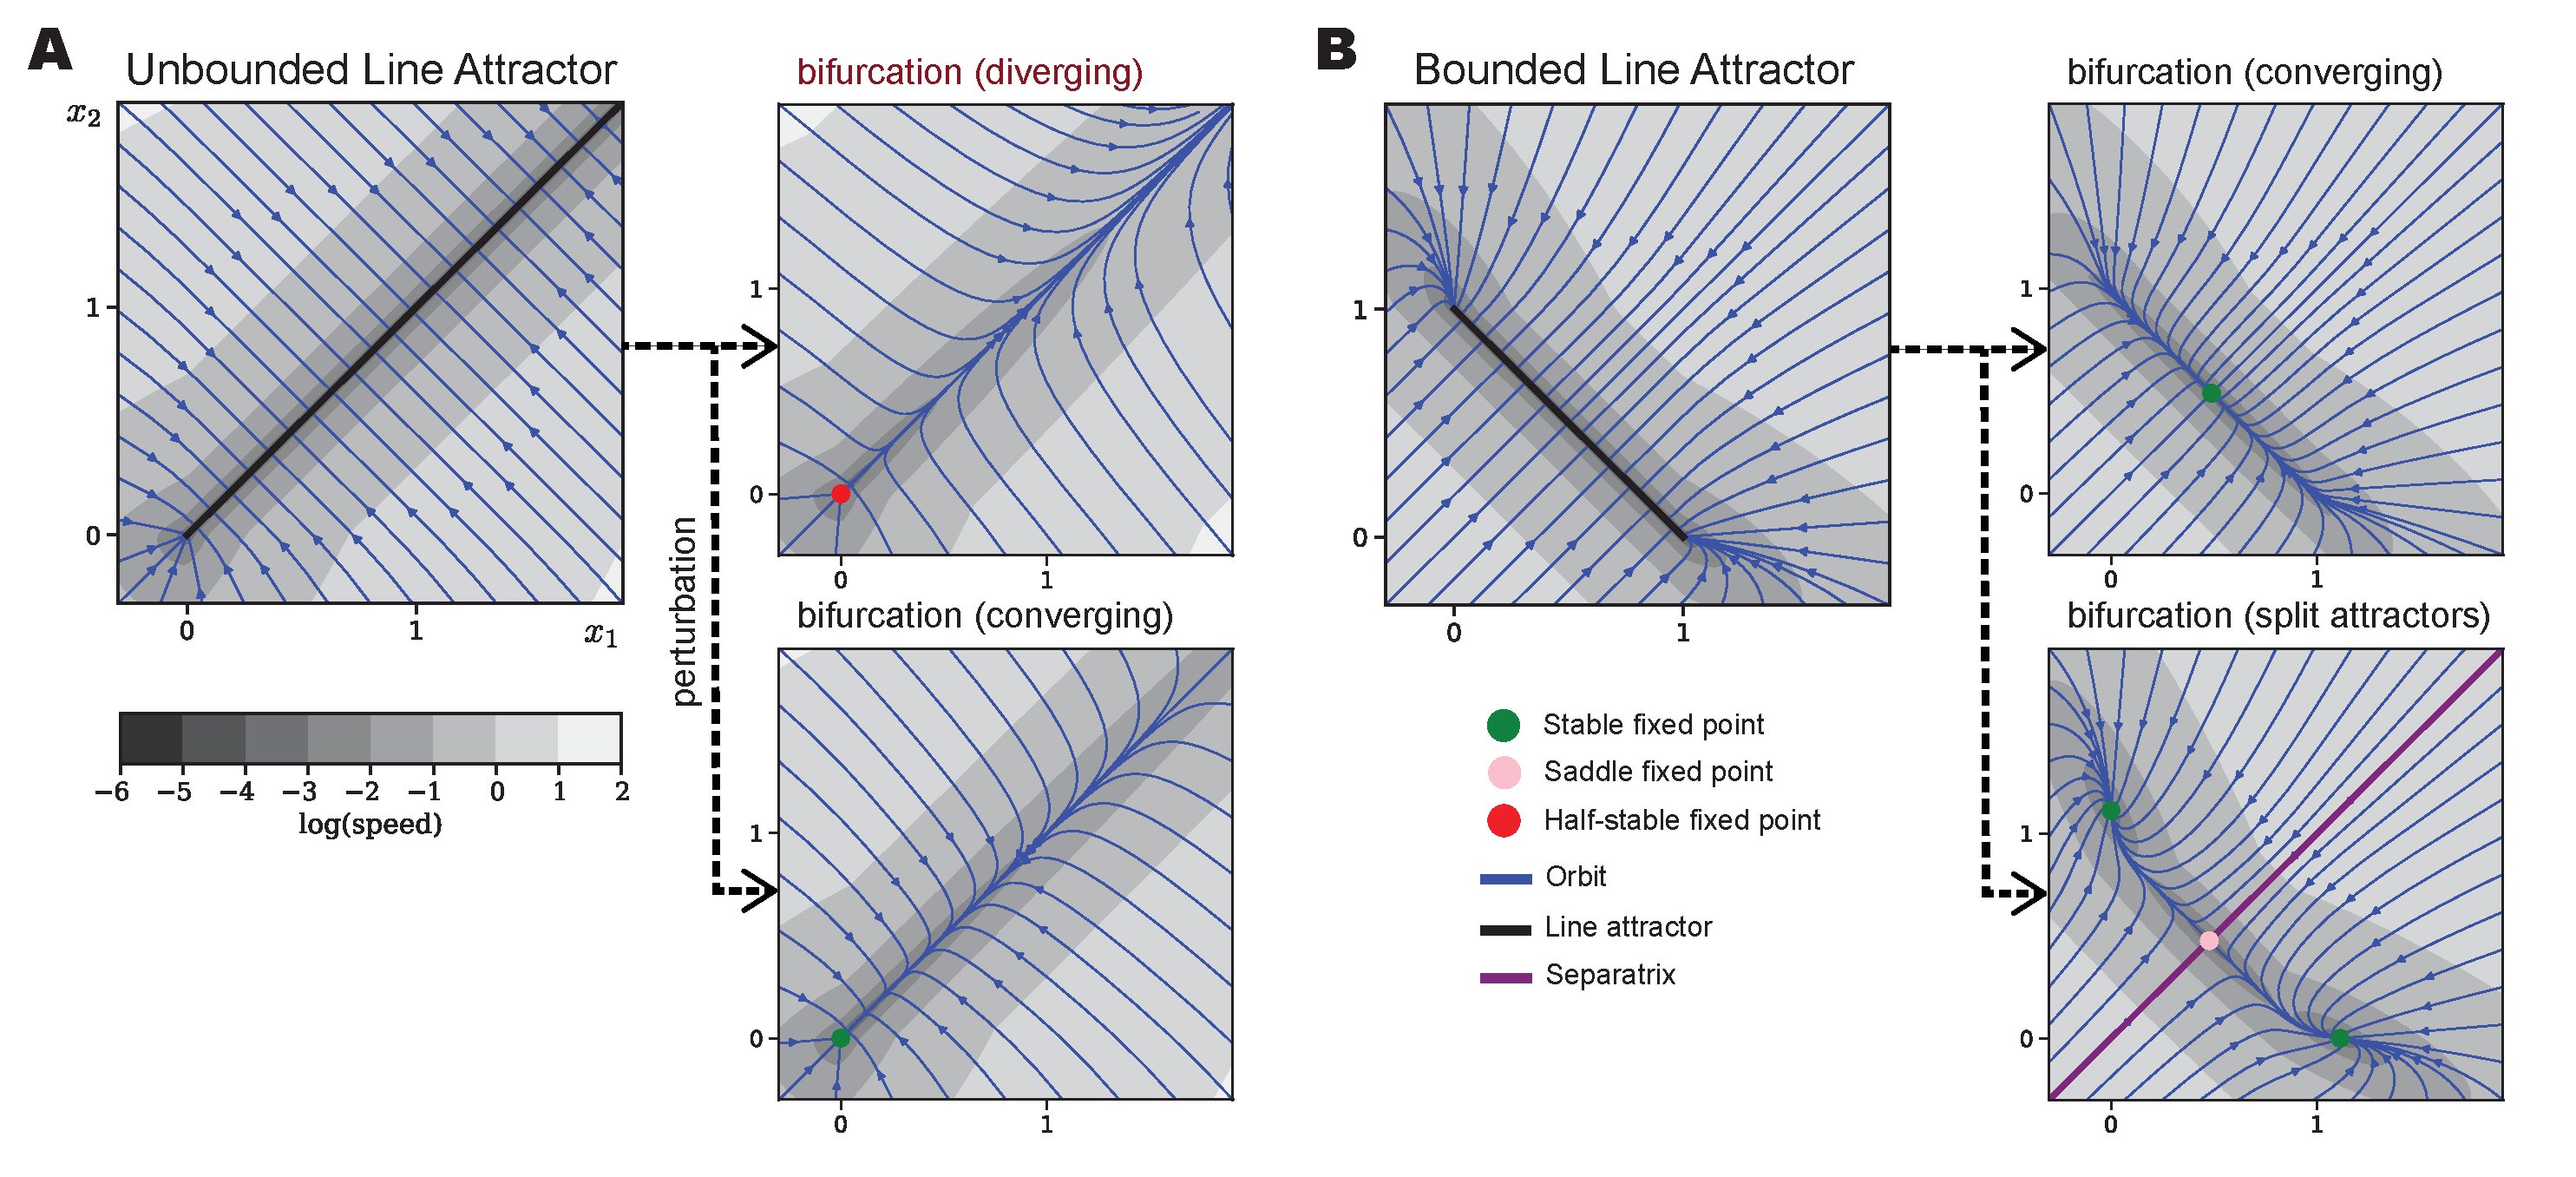
\includegraphics[width=\textwidth]{figures/UBLABLA}
  \caption{Motivating case study of the two systems implementing the same computation but one near exploding gradients.
    Phase portraits for unbounded and bounded linear attractors~\eqref{eq:TLN}.
    Under perturbation of parameters, each of them can bifurcate to one of the two potential systems without the continuous line attractor.
    Note that the parameters for the UBLA are near a diverging system associated with exploding gradient behavior.
% Behavior and bifurcations of the unbounded and bounded line attractors.  Some example orbits are shown with blue lines for each system while the log of the speed in state space is indicated with a grayscale gradient.
%   (Left) Example orbits  for a ReLU RNN implementation of an unbounded line attractor (black line, see Sec. ~\ref{sec:ubla}). This system can bifurcate in two types of dynamics. (Upper arrow) The first type of perturbation leads to a divergent systems with orbits going to positive infinity for all starting positions (except a single orbits that end up at the origin).
%    (Lower arrow) The second type of perturbation leads covergent dynamics with all orbits converging at the origin.
%  (Right from red line) Example orbits (blue lines) for a ReLU RNN implementation of an bounded line attractor (black line, see Sec ~\ref{sec:bla}). This system can bifurcate into two systems with non-zero probability.
%  (Upper arrow) The first type of perturbation leads to a system with a single fixed point (pink).
%  (Lower arrow) The second type of perturbation leads to a system with three fixed points.
}
  \label{fig:ublabla}
\end{figure}

Avoiding exploding gradients is of paramount importance in the context of long-range temporal learning (Sec.~\ref{sec:imp:ML}).
Learning generally induces stochasticity in parameters, while spontaneous synaptic fluctuations are present in biological neuronal networks (Sec.~\ref{sec:imp:neuroscience}).
Given these observations, we predict that BLA would be a more stable motif for computation than UBLA in the presence of noise and continuous learning.
Since BLA, but not UBLAs, avoids exploding gradients, if the desired computation requires a line attractor of finite range, BLA would be both easier to maintain and learn.
Is this only true for ReLU parameterized RNNs, or does it generalize?

In this paper, we lay out a new theory of general continuous-valued memory in the context of learning to answer the following questions:
\begin{enumerate}
    \item Can we avoid exploding gradients under parameter perturbation?
    \item Do we need to worry about the brittleness of the continuous attractor solutions in practice?
\end{enumerate}
Our theory provides answers to both questions under mild assumptions in an architecture agnostic manner.
Using Fenichel's invariant manifold theorem, we derive a sufficient condition for RNNs implementing continuous attractors to remain free of exploding gradients.
Moreover, even after a bifurcation, these RNNs still approximately behave like the original continuous attractor for a while.
Together these theoretical results practically nullify the concern of the fine tuning problem in theoretical neuroscience and suggest general principles for evaluating and designing new architectures and initialization strategies for RNNs in machine learning.

%\section{Background}
%\subsection{Dynamical systems and gradient propagation}
%\subsection{Structural stability and bifurcations}

\section{Theory of gracefully degrading continuous attractors}\label{sec:theory}
In this section, we apply Fenichel's work on invariant manifolds to RNNs and translate the results for the machine learning and theoretical neuroscience audience.

\subsection{Invariant Continuous Attractor Manifold Theory}\label{sec:imt}
We start by formulating RNNs implementing a continuous attractor in continuous time: $\dot{\vx} = \vf(\vx)$.
Let $l$ be the intrinsic dimension of the manifold of equilibria that defines the continuous attractor.
We will reparameterize the dynamics around the manifold with coordinates $\vy \in \reals^l$ and the remaining ambient space with $\vz \in \reals^{d-l}$.
To describe an arbitrary bifurcation of interest, we introduce a sufficiently smooth function $g$ and a bifurcation parameter $\epsilon \geq 0$, such that the following system is equivalent to the original ODE:
\begin{align}\label{eq:fenichel:flow}
    \dot{\vy} &=           \epsilon  \vg(\vy, \vz, \epsilon) \qquad \text{(tangent)}\\
    \dot{\vz} &= \hphantom{\epsilon} \vh(\vy, \vz, \epsilon) \qquad \text{(normal)}
\end{align}
where $\epsilon = 0$ gives the condition for the continuous attractor $\dot{\vy} = \mathbf{0}$.
We denote the corresponding manifold of $l$ dimensions $\manifold_0 = \{(\vy,\vz) \mid \vh(\vy,\vz,0) = 0\}$.

We need the flow normal to the manifold to be hyperbolic, that is \emph{normally hyperbolic}, meaning that the Jacobians $\nabla_\vz \vh$ evaluated on any point on the $\manifold_0$ has $d-l$ eigenvalues with non-zero real parts, and $\nabla_\vy \vg$ has $l$ eigenvalues with zero real parts.
More specifically, for continuous attractors, the real part of the eigenvalues of $\nabla_\vz \vh$ will be negative, representing sufficiently strong attractive flow toward the manifold.
Equivalently, for the ODE, $\dot{\vx} = \vf(\vx)$, the variational system is of constant rank, and has exactly $l$ eigenvalues with negative real parts and $(n-l)$ eigenvalues with zero real parts everywhere along the continuous attractor.

\begin{figure}[bthp]
  \centering
  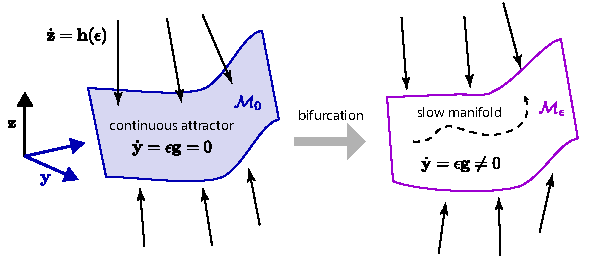
\includegraphics{figures/FenichelThm.pdf}
  \caption{
    Fenichel's invariant manifold theorem applied to compact continuous attractor guarantees the flow on the slow manifold is locally invariant and continues to be attractive.
    The dashed line is a trajectory ``trapped'' in the slow manifold (locally invariant).
  }
  \label{fig:fenichel}
\end{figure}

When $\epsilon > 0$, the continuous attractor bifurcates away.
What can we say about the fate of the perturbed system?
The continuous dependence theorem~\cite{Chicone2006} says that the trajectories will change continuously as a function of $\epsilon$ without a guarantee on how quickly they change.
Moreover, the topological structure and the asymptotic behavior of trajectories change discontinuously due to the bifurcation.
Surprisingly there is a strong connection in the geometry due to Fenichel's theorem~\cite{fenichel1971}.
We informally present a special case due to~\cite{Jones1995}:
\begin{theorem}[Fenichel's Invariant Manifold Theorem]
Let $\manifold_0$ be a connected, compact, normally hyperbolic manifold of equilibria originating from a sufficiently smooth ODE.
For a sufficiently small perturbation $\epsilon > 0$, there exists a manifold $\manifold_\epsilon$ diffeomorphic to $\manifold_0$ and locally invariant under the flow of \eqref{eq:fenichel:flow}.
Moreover, $\manifold_\epsilon$ has corresponding smoothness.
\end{theorem}

The manifold $\manifold_\epsilon$ is called the \emph{slow manifold} which is no longer necessarily a continuum of equilibria.
However, the local invariance implies that trajectories remain within the manifold except potentially at the boundary.
Furthermore, the non-zero flow on the slow manifold is slow and given in the $\epsilon \to 0$ limit as $\RN{\vy}{\tau} = \vg(c^\epsilon(\vy), \vy, 0)$ where $\tau = \epsilon t$ is a rescaled time and $c^\epsilon(\cdot)$ parameterizes the $l$ dimensional slow manifold.
In addition, the stable manifold(s) of $\manifold_0$ are similarly approximately maintained~\cite{Jones1995}, allowing the continuous attractor to remain attractive.

These conditions are met (up to numerical precision) for the BLA example in Fig.~\ref{fig:ublabla}B.
As the theory predicts, BLA bifurcates into a 1-dimensional slow manifold (dark colored regions) that contains fixed points, and overall still attractive.
On the contrary, the UBLA does not satisfy the compactness condition, hence the theory does not predict its persistence.
Importantly, the ``slow'' flow on the perturbed system is not bounded.

In practice, the sufficient conditions for RNNs implementing continuous attractors to have this graceful breakdown is for the continuous attractor manifold to be of finite dimension throughout, connected, and bounded. 
However, in systems with an invariant manifold with dimension at least three, it is possible that a slow manifold with chaotic dynamics is created through a perturbation. This would have as consequence that the perturbed system acquires positive Lyapunov exponents (corresponding to the chaotic orbit), which then can still lead to exploding gradients.

\subsection{Implications on Machine Learning}\label{sec:imp:ML}
Extending the memory time constant of RNNs have long been an important area of research with much focus on random weights~\cite{Legenstein2007,Goldman2009,Toyoizumi2011,Kerg2019,Chen2018,Henaff2016,Rusch2021,arjovskyUnitaryEvolutionRecurrent2016}.
Various initializations for the recurrent weights have been proposed to help learning: initialization with the identity matrix \citep{le2015}, with a random orthogonal matrix \citep{saxeExactSolutionsNonlinear2014,Henaff2016}, with a unitary matrix \citep{arjovskyUnitaryEvolutionRecurrent2016} and with a block diagonal weight matrix that creates a quasi-periodic system with limit cycles \citep{Sokol2019a}.
However, despite the capacity to maintain representation of continuous quantities for arbitrary duration of time, continuous attractor mechanism has not been pursued in machine learning research because of its brittleness.
The stochasticity in gradients inherited from the training data, regularization strategy, and multi-task learning objectives act as a perturbation on the recurrent dynamics, and continuous attractors break down even if it could be learned.
Remedies emerged in machine learning to hard-code continuous-valued memory structures within the RNNs---e.g., the cell state in vanilla LSTM.
However, our theory shows that the geometric structure of the manifold and the flow around the manifold play a critical role in enabling gradient descent learning of continuous attractors using standard methods such as backpropagation through time (BPTT)~\cite{Toomarian1991}.

It is well known that asymptotic exploding gradients comes from positive Lyapunov exponents~\cite{Mikhaeil2022,Vogt2022,Engelken2023}.
It has also been pointed out that bifurcations can cause arbitrarily large gradients~\cite{doya1993} as well as discontinuity in the Lyapunov spectrum~\cite{Park2023a}.
These gradient propagation theories suggested that bifurcations should be avoided, including the continuous attractors.

As far as we know, there is no architecture agnostic theory describing the loss landscape around RNN solutions.
We remark that due to the singular nature of the center manifold that supports the continuous attractor, the usual analysis approach of linearization fails.
\emph{Our theory successfully connects the invariant manifold theory and the gradient signal propagation theory in RNNs to describe two types of loss landscape around continuous attractor solutions.}
In one case, when the theorem holds, the landscape is shallow in all directions due to (asymptotically) vanishing gradients induced by the attractor structure---we have the gracefully degrading continuous attractor.
On the other case, we can find examples where the theorem does not hold, and the continuous attractor solution is at the boundary of network configurations with exploding gradients, meaning the loss landscape is very steep in some directions.

While exploding gradients would prevent gradient descent to correct for deviations from the optima,
for gracefully degrading ones, one can apply restorative forces via gradient descent to be in the vicinity of the brittle continuous attractor solution (see Sec.~\ref{sec:exp:maintaining}).


\subsection{Implications on Neuroscience}\label{sec:imp:neuroscience}
Continuous attractors are biologically plausible, theoretically elegant, consistent with neural recordings, and avoids the asymptotic exploding and vanishing gradient problem~\cite{Park2023a}.
As a conceptual tool in computational and theoretical neuroscience, continuous attractors are widely used when working memory of continuous values is needed~\cite{Dayan2001,Burak2009,Khona2022}.
When used to accumulate stimulus, continuous attractors are also called neural integrators that are hypothesized to be the underlying computation for the maintenance of eye positions, heading direction, self-location, target location, sensory evidence, working memory, decision variables, to name a few~\cite{seung1996,Seung2000,Romo1999}.
Neural representation of continuous values have been observed as persistent activity in the prefrontal cortex of primates, ellipsoid body of the fly, and hypothalamus~\cite{Romo1999,noorman2022,Nair2023}.
A typical computational implementation of a continuous attractor are bump attractor network models which require a mean-field limit~\cite{Skaggs1995,Camperi1998,Renart2003} and finite sized networks with threshold linear units \cite{noorman2022,Spalla2021}, see also Sec.~\ref{sec:hd}.

However, the so-called ``fine-tuning problem'' describing the theoretical and practical brittleness of continuous attractors was recognized in~\citep{seung1998}.
Since biological neural systems have constantly fluctuating synaptic weights~\cite{shimizu2021}, this has been a big puzzle in the field.
There have been efforts and remedies to lessen the degradation for particular implementations, often focusing on keeping the short-term behavior close to the continuous attractor case~\cite{Lim2012,Lim2013,Boerlin2013,Koulakov2002,Renart2003}.

Our theory shows that not all continuous attractors are born equal, and there are gracefully degrading continuous attractors.
In finite time, trajectories are well-behaved, contrary to the asymptotic behavior captured by the Lyapunov exponents.
Animal behavior is finite time in nature and the longer the temporal distance the harder it is to learn in general.
The conditions are favorable in the recurrent neuronal networks: (1) mutual inhibition is widely present and evidence points to inhibition dominated dynamics,
(2) the neural state space is bounded due to physiological constraints--non-negative firing rate and maximum firing rate.

%Given an $d$-dimensional continuous attractor manifold embedded within a recurrent dynamics of $n$-dimensions, it supports persistent continuous memory of $d$-dimension.
%There are $d$ zero Lyapunov exponents corresponding to the perturbations tangent to the manifold, coinciding with the memory representation, and $(n-d)$ negative Lyapunov exponents that expresses the attractive nature.
%In theory, the topology of the manifold can be arbitrary, ideally matching the desired structure of the target variables.

\section{Experiments}
\subsection{Continuous-valued click integration task}\label{sec:task:continuous-clicks}
Although there are several standard benchmark tasks for temporal dependence learning with memory components,
due to the discrete nature of the relevant stimulus space, the solutions do not necessarily require a continuously-valued memory.
We designed a simple integration task where one of the optimal solutions is the continuous attractor.

We extend the Poisson clicks task which has been used for studying perceptual decision making~\cite{bruntonRatsHumansCan2013}.
Neural integrators are considered to be crucial for the task for accumulating evidence over time and maintaining a continuous representation of the accumulated evidence.
For our experiments, we used discrete time representations over $T$ time bins and the real-valued\footnote{Approximated as single precision IEEE 754 floating point.} stimulus encoded as difference of two non-negative values:
\begin{align}
    I_{t,i} &= m_{t,i} \cdot u_{t,i} 
            & \qquad \text{(continuous clicks)}
    \\
    O^\ast_{t} &= \sum_{s=0}^{t} \left(
        I_{s,1} - I_{s,2}
        \right)
            & \qquad \text{(desired output)}
\end{align}
where $m_{t,i}$ are independent Bernoulli random variables with probability $0.2$ and $u_{t,i}$ are independent random variables with uniform distribution on the unit interval.
We used mean squared error (MSE) of the 1-dimensional output over time as the loss function over all time bins.
We used $T=500$ time bins per trial unless specified otherwise.
The gradients were computed in batch mode with $1000$ randomly generated trials.
The main challenges of this task are (1) addition and subtraction and (2) maintain the accumulated clicks for extended period of time.

%The inputs for the clicks task are incoming clicks in two channels ($K=2$) and are given as follows.
%The non-zero inputs follow a Poisson distribution with given rates.
%At such time points, an input is sampled from $[0,1]$.
%The task is to output the difference between the two inputs in the two channels. 

%A noisy version of the task also includes noise added to a part of the input, without alternation to the target output, i.e., the noise added to the system should be ignored by the system.

\subsection{RNN solutions to the integration task}\label{sec:rnn:integration}
We use vanilla RNN implementations with the standard parameterization:
%An RNN \citep{elmanFindingStructureTime1990} consists of a $N \times N$ transition matrix $W$, an $L \times N$ decoder matrix $\wout$ (where $L$ is the output dimension), a $N \times K$ encoder matrix $\win$ (where $K$ is the input dimension), and a bias $b$ for the hidden state and $\bout$ for the output.
% If either the output or input is categorical, $M$ (respectively $N$) is the number of classes, and we use a one-hot representation. 
%As the RNN ingests a sequence, at each timestep it updates to a hidden state $h$, and using the hidden state and the decoder matrix, produces outputs $y$:
\begin{equation}
  \begin{aligned}
	\vx_t &= \sigma(\win \vI_t + \vW \vx_{t-1} + \vb) \label{eq:RNN:discrete}\\
	O_t &= \wout \vx_t + \bout
  \end{aligned}
\end{equation}
where $\vx_t \in \reals^d$ is the hidden state, $\vI_t \in \reals^K$ is the input,
$\sigma: \reals \to \reals$ an activation function which acts on each of the hidden dimension, and
$\vW, \vb, \win, \wout, \bout$ are parameters.
Assuming an Euler integration with unit time step, the discrete-time RNN of \eqref{eq:RNN:discrete} corresponds to the ODE:
\begin{align}
    \dot{\vx} &= -\vx + \sigma(\win \vI + \vW \vx + \vb) \label{eq:RNN:continuous}
\end{align}

For tractable analysis, we consider $2$ dimensional systems with ReLU activation.
We study three different RNN implementations of an integrator, the Identity RNN (iRNN), UBLA and BLA.
On the original clicks task the UBLA and BLA networks count the click differences directly, while iRNN counts the clicks separately and then subtracts these representations through the output mapping.
The behaviors of UBLA and BLA in the absence of stimulus are shown in Fig.~\ref{fig:ublabla}, while the behavior of the iRNN is trivial since there is no flow. These networks are defined as follows.

\paragraph{Identity RNN}
\label{sec:ubpa,sec:iRNN}
%This is an RNN with the identity matrix as its recurrent weights  with two hidden units. 
\begin{equation}\label{eq:irnn}
\win = 
\begin{pmatrix}
1  &  0 \\
0 &  1
\end{pmatrix}, \
\vW = 
\begin{pmatrix}
1  &  0 \\
0  &  1
\end{pmatrix}, \
\wout = 
\begin{pmatrix}
-1  \\  1 
\end{pmatrix}, \
\vb = 
\begin{pmatrix}
0  \\ 0
\end{pmatrix}, \
\bout = 0.
\end{equation}

%The system has the whole state space as its invariant manifold.

\paragraph{Unbounded line attractor}
\label{sec:ubla}
\begin{equation}\label{eq:ubla}
\win = \alpha
\begin{pmatrix}
-1  &  1 \\
-1  &  1
\end{pmatrix}, \
\vW = 
\begin{pmatrix}
0  &  1 \\
1  &  0
\end{pmatrix}, \
\wout = \frac{1}{2\alpha}
\begin{pmatrix}
1  \\  1 
\end{pmatrix}, \
\vb = 
\begin{pmatrix}
0  \\  0
\end{pmatrix}, \
\bout = -\frac{\beta}{\alpha}.
\end{equation}

While the line attractor is unbounded from above, it only extends to the center from below.  The  step size along line attractor $\alpha$ determines the maximum number of clicks as the difference between the two channels; the capacity is $\beta/\alpha$ number of clicks.

\paragraph{Bounded line attractor}\label{sec:bla}
We formulate this implementation of a bounded integrator with a parameter that determines step size along line attractor $\alpha$. Analogously as for UBLA, these parameters determine the capacity of the network.
The inputs push the input along the line attractor in two opposite directions, see below. UBLA and BLA need to be initialized at $\beta(1,1)$ and $\tfrac{\beta}{2}(1,1)$, respectively, for correct decoding, i.e., output projection.

\begin{equation}\label{eq:bla}
\win = \alpha
\begin{pmatrix}
-1  &  1 \\
1  &  -1
\end{pmatrix}, \
\vW = 
\begin{pmatrix}
0  &  -1 \\
-1  &  0
\end{pmatrix}, \
\wout = \frac{1}{2\alpha}
\begin{pmatrix}
1  \\  -1 
\end{pmatrix}, \
\vb = \beta
\begin{pmatrix}
1 \\  1 
\end{pmatrix}, \
\bout = 0.
\end{equation}

\subsection{Asymmetric loss landscape due to exploding gradients}
To illustrate the effect of bifurcations from continuous attractor solution, we take a 1-dimensional slice of the loss surface.
Specifically, we take the self-recurrent connection and systematically vary:
\begin{align}
    \vW_{1,1} \leftarrow \vW_{1,1} + \Delta.
\end{align}
The result is shown in Fig.~\ref{fig:maintenance}A.
For UBLA and iRNN, positive perturbations shows exponentially increasing loss due to the bifurcation to an exploding gradient dynamical system.
In all other cases, including all perturbations of BLA, leads to vanishing gradient, hence the loss is bounded.

\begin{figure}[thbp]
  \centering
  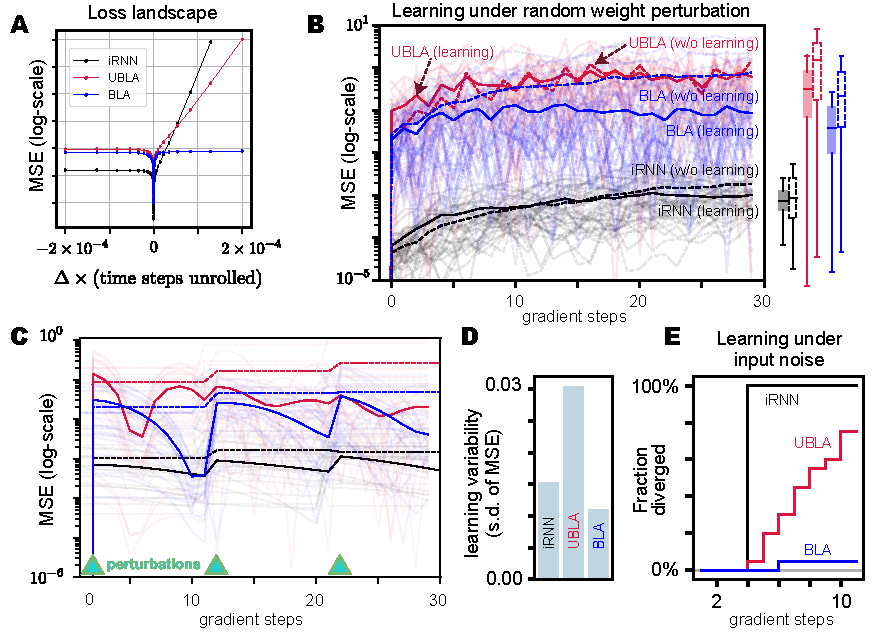
\includegraphics[width=\textwidth]{figures/threeIntegrators.pdf}
  \caption{
  Comparing three continuous attractor solutions to the clink integration task.
  (A) Single parameter perturbation showing exploding gradients for iRNN and UBLA.
  (B) Effect of gradient descent in repairing the continuous attractor. RNNs without gradient descent (dashed line) are shown for reference. Box plots show distribution of the loss for the last 10 steps.
  (C) Interleaved weight perturbations showing gradual recovery for BLA and iRNN.
  (D) High variability across time of UBLA and iRNN due to exploding gradients.
  (E) Noise injected to objective induces gradient descent to drive solutions to diverge away.
  }
  \label{fig:maintenance}
\end{figure}


\subsection{Bifurcation probability and random perturbations}
We consider all parametrized perturbations of the form $ \vW \leftarrow \vW + \vV$ for a random matrix $\vV\in \mathbb{R}^{2\times 2}$.
The BLA can bifurcate in the following systems, characterized by their invariant sets: a system with single stable fixed point, a system with three fixed points (one unstable and two stable) and  a system with two fixed points (one stable and the other a half-stable node) and a system with a (rotated) line attractor. 
Only the first two bifurcations (Fig. ~\ref{fig:ublabla}) can happen with nonzero chance for arbitrary the type of perturbations we consider.
The  perturbations that  leave the line attractor intact and or two a system with two fixed points have measure zero in parameter space.
The types of perturbation with measure zero are codimension 2 bifurcations.
The perturbation that results in one fixed point happen with probability $\frac{3}{4}$, while perturbations lead to a system with three fixed points with probability $\frac{1}{4}$.




\subsection{Maintaining a neural integrator}\label{sec:exp:maintaining}
To investigate the differential effect of gradient descent on the three neural integrator models, we performed three learning experiments using the continuous-valued click integration task.

In the first experiment, Gaussian random noise is injected to all parameters inducing a constant diffusion of the parameters.
This emulates the biological synaptic variability.
Fig.~\ref{fig:maintenance}B shows that for BLA, gradient descent (with constant learning rate, chosen from a grid search) was able to counter the diffusion.
Note that the magnitude of perturbation were identical for all networks, but iRNN is more robust in terms of MSE.
The distribution of MSE for the task can be used as proxy for the misadjustment from the optimal solution.
BLA with learning has superior misadjustment to UBLA and BLA without learning.

To dissociate the effect of misadjustment from gradient descent and external perturbation, we interleaved a larger perturbation with 10 gradient steps.
Fig.~\ref{fig:maintenance}C shows consistent learning in the average MSE for BLA and iRNN, but not in UBLA.
The individual runs indicate larger variability induced by learning over time, which we quantify in Fig.~\ref{fig:maintenance}D.
iRNN and UBLA both have larger learning noise than BLA, consistent with the absence of exploding gradient configuration around the optimum.

Finally, we investigated the effect of learning when perturbations are induced by the backpropagated gradient which is structured by the recurrent dynamics.
To inject noisy gradients naturally, we added noise to the input to the first 10 time steps during the trial that were not integrated.
Then we looked for networks that diverged due to exploding gradients which we identify as having a loss of 1 or higher. %normally loss is very low, zero for the perfect integrators
Fig.~\ref{fig:maintenance}E shows that UBLA and iRNN quickly diverges under gradient descent than the BLA.
%$This is because the noise sometimes pushes the UBLA to the regime with divergent dynamics which leads to exploding gradients, which then causes the weights to make bigger jumps.


%noisy learning experiments
%We investigate the effects of noise to the inputs on the loss and the effect of such noise on the learning/adjustment of the parameters during gradient descent starting from the perfect solutions to the task.
%We inject a pulse of 10 steps of inputs sampled from the uniform distribution and take a gradient step in the direction of the accumulated gradient.

The parameters that were used for the effects of input- and parameter-type noise are summarized in Table \ref{tab:params}.
The bias parameters of the UBLA and BLA networks were set to $\beta=100$, while $\alpha=1$. 
The hidden state at the beginning of a trial is a learnable parameter. 
The optimal learning rates for the input-type noise experiments were chosed from a set of three values ($\{10^{-8},10^{-9},10^{-10}\}$) based on best performance of the task of 20 runs.

A sequence of inputs is generated of maximum length $T_I$ generated as described above. 
For the experiments with D-type noise, we generate noise in the input for a sequence length of 10 time steps and distribution width sampled from the uniform distribution $(-\sigma,\sigma)$ with $\sigma=10^{-6}$.
For the experiments with S-type noise, we perturb the weights with a matrix with entries sampled from $\mathcal{N}(0, \sigma)$.
We inject this noise into the system either after each learning epoch (Fig. \ref{fig:maintenance}B) or in pulses only at epochs 1,11 and 21 (Fig. \ref{fig:maintenance}C).
The first experiment should demonstrate the effects of the restorative force of learning.

\begin{table}
\caption{Summary of parameters for experiments.}\label{tab:params}
\centering
\bgroup
\def\arraystretch{1.52}
\begin{tabular}{|c||c|c|}
\hline
Parameter     &  Input noise & Paramter noise \\\hline \hline
Trial length (time steps)	 &    200   & 500			\\\hline 
Input sequence length ($T_I$) &		100 & 50   \\\hline
Learning rate\footnote{The optimal value of $10^{-10}$ was used for the parameter noise for UBLA and BLA for the interleaved perturbation experiment. } &	 		$10^{-4}$   &  $10^{-9}$\\\hline 
Perturbation	parameter ($\sigma$) &		$10^{-6}$   & $10^{-5}$\\\hline 
\end{tabular}
\egroup
\end{table}







\subsection{Perturbation of continuous attractors}
%We will now investigate the effects that perturbations might have on the gradients in some continuous attractor network models used in computational neuroscience.



%\subsubsection{Ring attractor}

%Compact
%No boundary: in- and outflowing
%But not $C^1$!


%discrete attractors as a trivial application?
%Discrete attractors can be seen as an approximation to continuous attractor models in the context of head direction representation \citep{zhang1996}. The discrete nature of the representation makes it more robust to small fluctuations or disturbances in neural activity.
%However, these system have fading memory: the system eventually forgets the past, since any difference between any two neural activations eventually tends zero as they both evolve to a global resting state.

We will first of all look at a simple (non-biological) system that has a ring attractor to demonstrate the consequences of the Persistence Theorem.
The system we will analyse is defined by the following ODE: $\dot r = r(1-r), \ \dot \theta = 0.$
This system has as fixed points the ring with radius one centered around zero, i.e., $(0,0)\cup\{(1,\theta)\ |\ \theta\in[0,2\pi)\}$.




\begin{figure}[H]
     \centering
  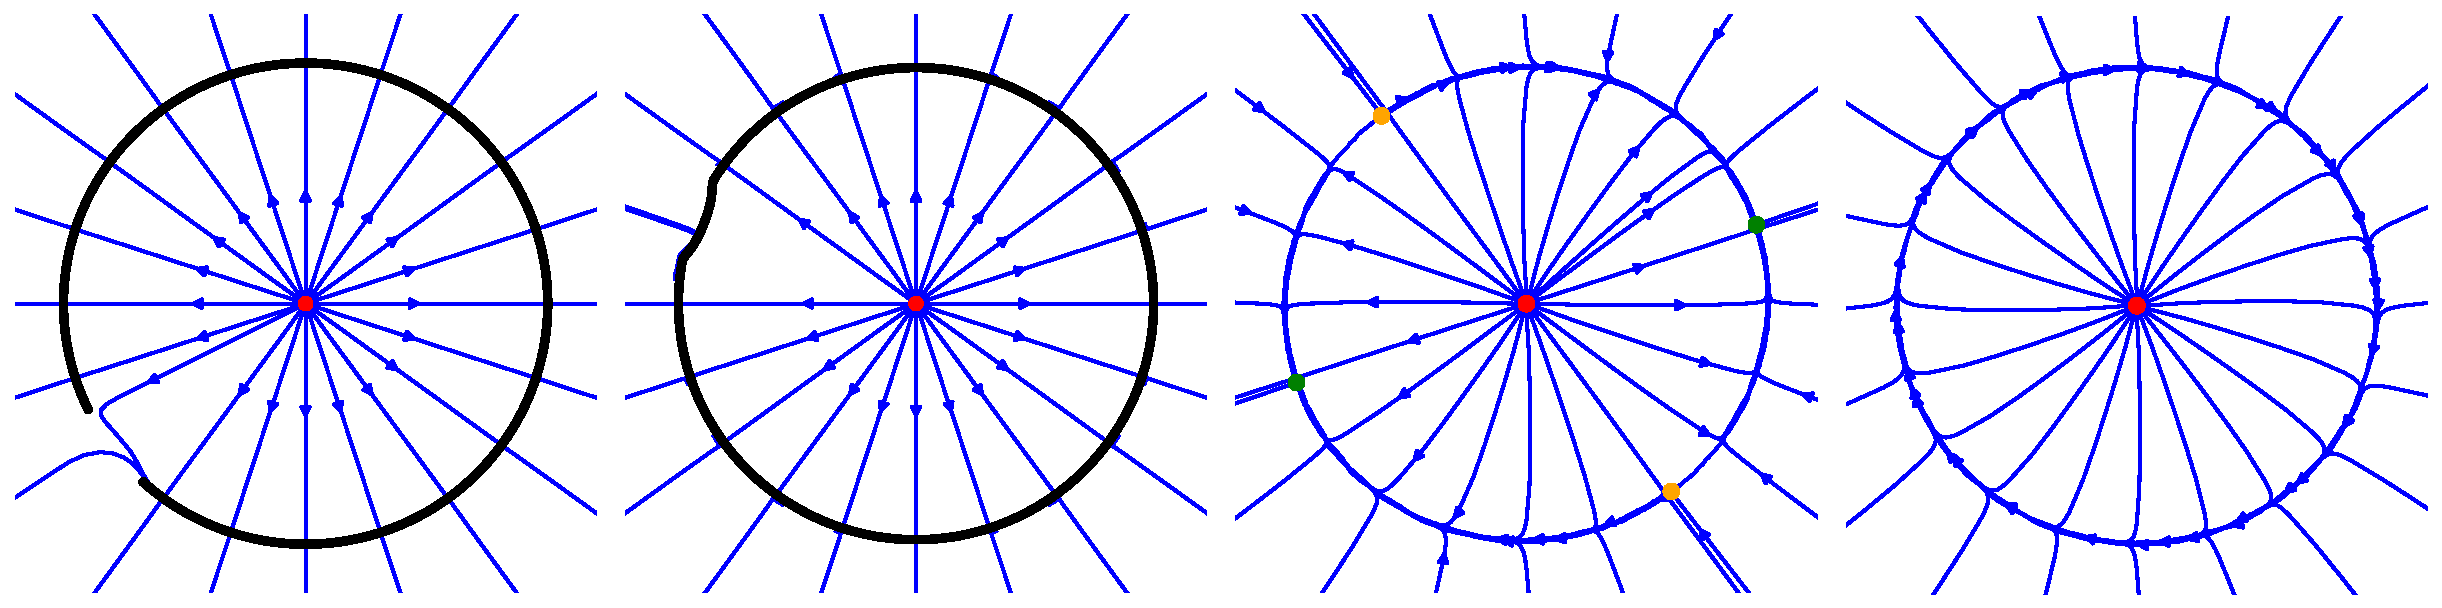
\includegraphics[width=\textwidth]{figures/ring_perturbations_stream}
       \caption{Perturbations to a simple implementation of a ring attractor all leave the invariant manifold intact. (Left)  Examples of a local perturbation to the vector field through the addition of a bump to the vector field along the ring attractor.
              (Leftmost) An example of a bump perturbation that results in the ring breaking up and becoming diffeomorphic to a line. %slow flow in hole?
              (Left, middle) An example of a bump perturbation that maintains the ring structure, but deforms it locally.
              %
       (Right) Examples of a global perturbation to the vector field through the addition of a small term to the connectivity matrix. 
       (Right, middle) A global perturbation that results in a system with four fixed points along the persistent invariant manifold. The two saddle nodes (yellow dots) are connected to the stable fixed points (green dots) through connecting orbits.
       (Rightmost)   A global perturbation that results in a limit cycle.}
         \label{fig:ring_activity_pert}
\end{figure}

%All perturbations maintain the invariant manifold.



\subsubsection{Finite-sized head direction network model}\label{sec:hd}
Continuous attractor models of the head direction representation suggest that the representation emerges from the interactions of recurrent connections among neurons that form a circular or ring-like structure \citep{zhang1996, noorman2022, ajabi2023}. 
Since continuous attractors are susceptible to noise and perturbations the precise representation of the head direction can in principle easily be disrupted.
We will the implications of the Persistence theorem in the case of the implementation of a continuous ring attractor presented in \citep{noorman2022}.
As this continuous ring attractor is bounded its invariant manifold persists and, hence, no divergent orbits are created under small perturbations to this system.
This model is composed of $N$ heading-tuned neurons  with preferred headings $\theta_j \in \{\frac{2\pi i}{N}\}_{i=1\dots N}$ radians.
For sufficiently strong local excitation (given by the parameter $J_E$) and broad inhibition, this network will generate a stable bump of activity, one corresponding to each head direction. This continuum of fixed points for a one dimensional manifold homeomorphic to the circle. 

\begin{figure}[H]
     \centering
  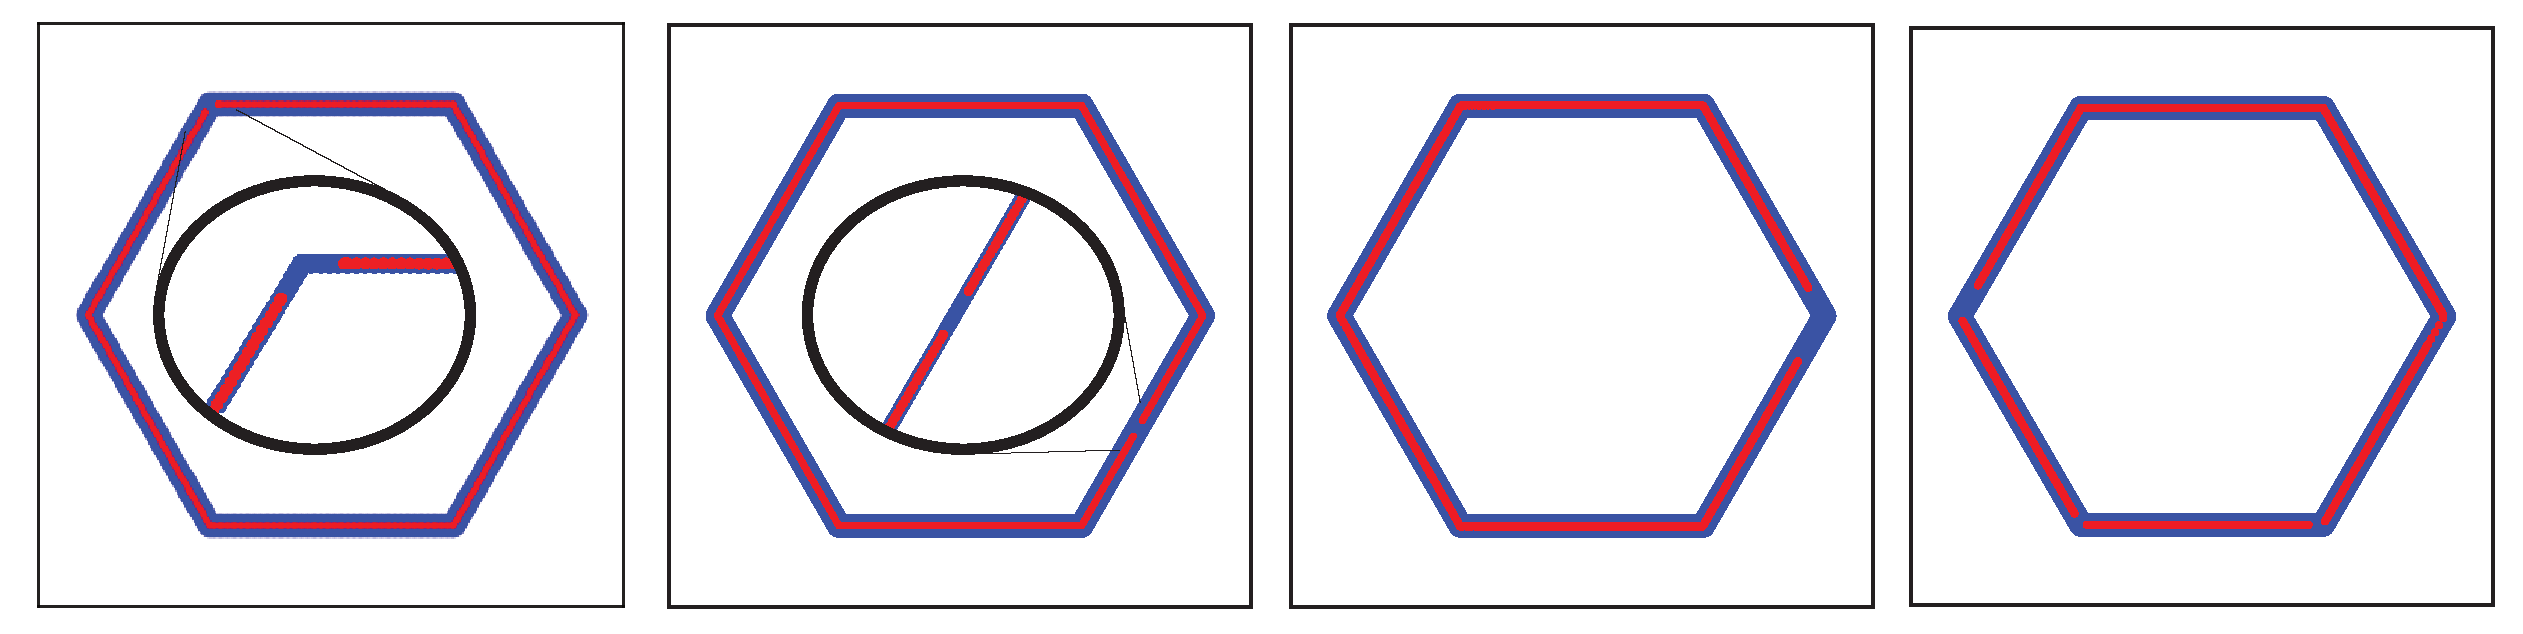
\includegraphics[width=\textwidth]{figures/noorman_perturbations}
       \caption{Perturbations to the ring attractor introduced in \citep{noorman2022}. (Left)  Examples of a local perturbation to the vector field through the addition of a bump to the vector field along the ring attractor.
       (Leftmost) An example of a bump perturbation which cuts out a piece of the ring attractor, the stable fixed points of the system are shown in black. A heteroclinic orbit is created on the bounday of the hole with a slow flow.
       (Left, middle) An example of a bump perturbation that deforms the ring attractor, but maintains its topology.
       (Right) Examples of a global perturbation to the vector field through the addition of a small term to the connectivity matrix. }
         \label{fig:noorman_ring_activity_pert}
\end{figure}


We evaluate the effect of perturbations on a network of size $N = 6$ with the optimal value $J_E^*=2.4$ through local and parametrized perturbations, similarly as for the toy ring attractor model.
The space of possible perturbations in Sec. ~\ref{sec:imt} is very large. To be able to form an image of what happens in the theorem we will work out the effect of some examples of perturbations. Hereby, we will focus on two kinds of perturbations, local and parametric. 
%Definition of a bump perturbation
We define a local perturbation (i.e., a change to the ODE with compact support) through the bump function $\Psi(x) = \exp\left(\frac{1}{\|x\|^2-1}\right)$ for $\|x\|<1$ and zero outisde, by multiplying it with a uniform, unidirectional vector field. 
%Definition of a global perturbationThe parametrized perturbations are characterized as the addition of random matrix to the connection matrix. 
We further investigate the effect of parameteric perturbations of the form if a term $\vW x$ to the original ODE with the entries of $\vW$ sampled from a normal distribution with mean zero and variance $\frac{1}{100}$. 
All such perturbations leave at least a part of the continuous attractor intact and preserve the invariant manifold, i.e. the parts where the fixed points disappear a slow flow appears.





\section{Discussion}
We have derived a general theory that describes the loss landscape of RNNs around continuous attractor solutions.
This theory implies backpropagating gradient does not explode for systems near compact continuous attractors because of divergent dynamics.
This insight also suggests that there can exist homeostatic mechanisms for certain implementations of continuous attractors that maintain the structure of the attractor sufficiently for the neural computation it is used in, which we demonstrate in simple networks.

%activation functions
It is well-known that activation functions play a critical role in propagating these gradients effectively through the network  \citep{jagtap2022, ramachandran2017, hayou2019}.
The activation function can have many forms.
The ones that are $C^r$ for $r\geq 1$ are the ones to which the Persistence Theorem applies. 
The Persistence Theorem further specifies how the smoothness of the activation can have implications on the smoothness of the persistence invariant manifold.
For situations where smoothness of the persistent invariant manifold is of importance, smoother activation functions might be preferrable, such as the Exponential Linear Unit (ELU)\citep{clevert2016} or the Continuously Differentiable Exponential Linear Units (CELU) \citep{barron2017}.




%\subsection{Footnotes}
%Footnotes should be used sparingly.  If you do require a footnote, indicate
%footnotes with a number\footnote{Sample of the first footnote.} in the
%text. Place the footnotes at the bottom of the page on which they appear.
%Precede the footnote with a horizontal rule of 2~inches (12~picas).
%
%
%Note that footnotes are properly typeset \emph{after} punctuation
%marks.\footnote{As in this example.}

%\begin{ack}
%Use unnumbered first level headings for the acknowledgments. All acknowledgments go at the end of the paper before the list of references. Moreover, you are required to declare
%funding (financial activities supporting the submitted work) and competing interests (related financial activities outside the submitted work).
%More information about this disclosure can be found at: \url{https://neurips.cc/Conferences/2023/PaperInformation/FundingDisclosure}.
%
%
%Do {\bf not} include this section in the anonymized submission, only in the final paper. You can use the \texttt{ack} environment provided in the style file to autmoatically hide this section in the anonymized submission.
%\end{ack}



%\section{Supplementary Material}
%
%Authors may wish to optionally include extra information (complete proofs, additional experiments and plots) in the appendix. All such materials should be part of the supplemental material (submitted separately) and should NOT be included in the main submission.


%\section*{References}
%The natbib package will be loaded for you by default. Citations may be author/year or numeric, as
%long as you maintain internal consistency. As to the format of the references themselves, any style is
%acceptable as long as it is used consistently

%References follow the acknowledgments in the camera-ready paper. Use unnumbered first-level heading for
%the references. Any choice of citation style is acceptable as long as you are
%consistent. It is permissible to reduce the font size to \verb+small+ (9 point)
%when listing the references.
%Note that the Reference section does not count towards the page limit.
%\medskip

\small

\newpage
\bibliographystyle{plain}
\bibliography{cit,CITCOD,CITCom,catniplab}

\newpage
\section{Supplementary Material}

RNNs are also capable of learning complex patterns and relationships in the data, which makes them in particular useful as models for neural computations. This is achieved through the use of non-linear activation functions and the training of the network using backpropagation through time (BPTT).
BPTT allows the network to adjust the weights of the connections between neurons based on the error signal that is propagated backwards through time. 
%This makes them suitable models for 

However, training RNNs by using back-propagation through time to compute error-derivatives can be difficult.  Early attempts suffered from vanishing and exploding gradients \citep{kolenGradientFlowRecurrent2009} and this meant that they had great difficulty learning long-term dependencies. 
Many different methods have been proposed for overcoming this difficulty.

%
%\vspace*{5cm}
%
%RNNs are also capable of learning complex patterns and relationships in the data, which makes them in particular useful as models for neural computations. This is achieved through the use of non-linear activation functions and the training of the network using backpropagation through time (BPTT).
%BPTT allows the network to adjust the weights of the connections between neurons based on the error signal that is propagated backwards through time. 
%%This makes them suitable models for 
%
%However, training RNNs by using back-propagation through time to compute error-derivatives can be difficult.  Early attempts suffered from vanishing and exploding gradients \citep{kolenGradientFlowRecurrent2009} and this meant that they had great difficulty learning long-term dependencies. 
%Many different methods have been proposed for overcoming this difficulty.
%%
%Exploding gradients occur when the gradients in a neural network become very large during training.  In RNNs, this problem arises because the gradients can be multiplied many times as they are passed through the recurrent connections. This can cause the weights to be updated with very large values, leading to numerical instability and poor performance.
%%
%The issue with exploding gradients is that the weight updates become too large to be useful. When the gradients become very large, the weight updates can become so big that they overshoot the optimal weights, causing the network to diverge and perform poorly. In extreme cases, the weight updates can be so large that they cause the weights to overflow, resulting in numerical errors. Even worse, in case the gradients arise from some noise, the gradient descent algorithm can drift far away from the optimal weights throught the explosion in the gradients.
%
%To prevent exploding gradients in RNNs, a common approach is to use gradient clipping, where the gradients are scaled down when they exceed a certain threshold. This ensures that the weight updates remain within a reasonable range and prevents numerical instability. Additionally, techniques like weight initialization, regularization, and adaptive learning rate methods can also be used to improve the stability of the training process and prevent the occurrence of exploding gradients. However, these measures either do not fully solve the fundamental issues with exploding gradients or would be very difficult to implement in a biological neural network.
%
%Instead, we use Neil Fenichel's persistence theorem to show that networks relying on a bounded (continuous) attractor are not sensitive to perturbations in a way that would create unstable systems (with orbits diverging to infinity).
%In simple terms, the theorem states that if a dynamical system has a normally hyperbolic invariant manifold, which is a type of geometric structure that characterizes the system's behavior near an equilibrium or periodic orbit, then this structure persists under small perturbations of the system's parameters or equations. In other words, the system's behavior remains qualitatively the same despite the perturbation, and nearby trajectories follow trajectories that are close to the original invariant manifold.
%
%Based on this result, we propose a new initialization of recurrent weights that has the same functionality as the identity initialization but does not have any systems in its neighbourhood with divergent dynamics that leads to exploding gradients.
%Further, we claim that for such systems there can exist a homeostatic mechanism that maintains the attractor through a restorative learning signal, something that is not possible for unbounded continuous attractors.
%
%\section{Background}
%%\subsection{RNNs}
%Recurrent neural networks (RNNs) are very powerful dynamical systems and they are the natural way of using neural networks to map an input sequence to an output sequence \citep{lipton2015, yu2019, sherstinsky2020}. We are mostly interested in tasks which require a memory of (continuous) variables which need to be maintained for arbitrarily long temporal delays. 
%The optimal implementation of a finite size network that can perform such tasks has to rely on a continuous attractor.
%Such dynamics are in particular difficult to learn through gradient descent and maintain in a noisy environment because of exploding gradients caused by bifurcations under perturbations to the continuous attractor. 
%We will see that while for unbounded continuous attractors (such as the identity matrix initialization in \citep{le2015}) noise under gradient descent is especially problematic, instability issues can be overcome with a restorative learning signal in bounded continuous attractor networks.
%
%%A Critical Review of Recurrent Neural Networks for Sequence Learning \citep{liptonCriticalReviewRecurrent2015}
%%
%%A Review of Recurrent Neural Networks: LSTM Cells and Network Architectures \citep{yuReviewRecurrentNeural2019}
%%
%%Fundamentals of RNNs \citep{sherstinskyFundamentalsRecurrentNeural2020}
%
%
%
%
%
%
%\subsection{Remembering continuous variables for a long time: Continuous attractor networks}
%%Attractors
%%An \emph{attractor} for a flow is a subset of the phase space of the system, which is invariant under the flow of the system and toward which nearby trajectories of the system converge over time.
%
%
%Continuous attractors are characterized by a continuum of equilibria that forms a manifold such as a line, a ring, or a plane, such that small perturbations away from the manifold asymptotically returns to the manifold.
%Continuous attractors can be used in a mechanism that integrates in combination with input pushing the activity along the attractor. Such integrators are hypothesized to be the underlying computation for the maintenance of eye positions, heading direction, self-location, target location, sensory evidence, working memory, decision variables, to name a few~\cite{seung1996}. %observed in flies?
%Since there is a continuum of stable equilibria where the neural activity does not change over time, the observed autonomous dynamics of the system is similar to a point attractor system, i.e., it generally decays to a fixed state and maintains constant activity over time.
%A key signature of a continuous attractor is persistent neural activity that can be maintained at any arbitrary level during any memory or delay period~\cite{romoNeuronalCorrelatesParametric1999,brodyBasicMechanismsGraded2003}.
%In neuroscience, a commonly used implementation of a continuous attractor are bump attractor network models~\cite{Renart2003,noorman2022}.
%
%
%Continuous attractor dynamics often suffer from the \emph{fine-tuning problem}---small change in the parameters can drastically reduce the effectiveness~\citep{seung1998}. 
%The fact that the realization of continuous attractors is fragile to parameter changes attractors means that such systems are structurally unstable, see Sec. ~\ref{sec:ss}.
%
%
%
%
%We review some standard recurrent neural network (RNN) implementations for processing sequential data suitable for long term memory.
%An exact line attractor can be easily designed and implemented, for example, linear dynamical system with null eigenvalues and Long short-term memory (LSTM) with no forgetting.
%%identity
%%unitary (QTPA)
%
%
%
%\subsection{Gradient descent and bifurcations}
%%\subsubsection{Exploding/Vanishing Gradient Problem (EVGP)}
%
%Gradient descent is a widely used optimization algorithm for minimizing the loss function of machine learning models. It works by iteratively updating the model parameters in the direction of the steepest descent of the loss function. 
%However, the performance of gradient descent can be hampered by the problem of exploding or vanishing gradients (i.e. the Exploding/Vanishing Gradient Problem (EVGP)).
%
%If a gradient descent algorithm with a fixed learning rate is used, a very large error gradient causes a long jump in the parameter space.
%Accumulating a very large error gradient can even lead to a numerical overflow. 
%Gradient descent does not work effciently when the size of gradient is magnitudes of order bigger in certain directions.
%In the case of exploding gradients, the gradient descent can end up in an orbit of oscillating weights.
%
%The exploding gradient problem occurs when the gradient of the loss function with respect to the model parameters becomes too large. This can cause the model parameters to update in a way that overshoots the optimal solution, leading to unstable training and poor performance. On the other hand, the vanishing gradient problem occurs when the gradient becomes too small, making it difficult for the model to learn long-term dependencies in the input data.
%
%%bptt already mentioned earlier
%Backpropagation through time (BPTT) is a widely used algorithm for computing gradients in (RNNs). It works by unrolling the RNN over time and applying the standard backpropagation algorithm to the resulting computational graph.
%In BPTT gradients tend to either blow up or vanish the temporal evolution of the backpropagated error exponentially depends on the size of the weights. This can make it difficult to train RNNs to learn long-term dependencies in sequential data.
%
%Learning equations used for error gradient estimation can be unstable because of certain bifurcations \citep{doya1993}.
%In dynamical systems, when infinitely small change in the parameters cause a qualitative change in the dynamics due to changes in the topology of the dynamics, it is said that the system undergoes a bifurcation.
%The asymptotic behavior of a recurrent neural network changes qualitatively at certain points in the parameter space, which are known as \emph{bifurcation points}.
%For example, a stable fixed point can change into an unstable fixed point or even disappear.
%At bifurcation points, the output of a network can change discontinuously with the continuous change of parameters and therefore convergence of gradient descent algorithms is not guaranteed in such cases.
%Continuous attractors are especially problematic because they lie on bifurcation points.
%
%
%
%
%\section{Stability}
%
%There exists two main types of stability analysis: local and global. Local stability analysis focuses on the behavior of a system near a specific equilibrium point or trajectory, and aims to determine whether small perturbations to the system will cause it to converge towards the equilibrium or diverge away from it. Global stability analysis, on the other hand, considers the behavior of the system over its entire state space, and aims to determine whether the system will converge to a particular attractor or exhibit more complex, chaotic behavior.
%
%Previous investigations into the stability properties of neural networks have mostly considered the (hyperbolic) stability of fixed points. In such analyses, given a nonlinear system with specified asymptotically stable equilibria,  the question is under what conditions will a perturbed model of the system possess asymptotically stable equilibria that are close (in distance) to the asymptotically stable equilibria of the unperturbed system \citep{wangRobustnessPerturbationAnalysis, zhangComprehensiveReviewStability2014}. 
%%Stability analysis review \citep{zhangComprehensiveReviewStability2014}
%
%
%\subsection{Structural stability of dynamical systems}\label{sec:ss}
%%what is never preserved in CANNs
%%\emph{SS is never preserved in CANNs}
%
%Biological neural systems have constantly fluctuating synaptic weights~\cite{shimizu2021}. %dendritic spine sizes, or their corresponding synaptic weights, are highly volatile even in the absence of neural activity
%In other words, there is noise in the recurrent network dynamics, which we call \emph{D-type noise}.
%
%An important consequence of the presence of D-type noise is that the neural dynamics of the network is constantly fluctuating.
%Therefore, the desirable properties of the dynamical system that require precise weight combinations are not stably achievable due to their unreliability.
%The topological structures that are robust under D-type noise are called \emph{structurally stable} -- for example, a stable fixed point is structurally stable~\cite{kuznetsovElementsAppliedBifurcation}.
%
%%\begin{definition}
%%    If $\mathcal{D}$ is the set of self-diffeomorphisms of a compact smooth manifold $M$, and $\mathcal{D}$ is equipped with the $C^1$ topology then $f\in\mathcal{D}$ is structurally stable if and only if for each g in some neighborhood of $f$ in $\mathcal{D}$ there is a homeomorphism $h\colon M\rightarrow M$ such that
%%\begin{equation}
%%\begin{tikzcd}
%%M \arrow[r, "f"] \arrow[d, "h" left] 
%%& M \arrow[d, "h"] \\
%%M \arrow[r, "g"]
%%& M
%%\end{tikzcd}
%%\end{equation}
%%commutes.
%%\end{definition}
%%That is, $f$ is topologically conjugate to each nearby $g$.
%
%Unfortunately, continuous attractors are not structurally stable -- small changes in the dynamical system can destroy continuous attractors, and as a consequence, the corresponding Lyapunov exponent(s) move away from zero.
%For example, in machine learning, vanilla RNNs are sometimes initialized at the continuous attractor regime with all zeros  which avoids the asymptotic EVGP initially, but very quickly loses the continuous attractor after one gradient step.
%This is a well known problem in neuroscience, often referred to as the ``fine tuning problem'' of the continuous attractor~\cite{seung1996,Renart2003,noorman2022}.
%
%
%
%\subsection{Persistence of invariant manifolds}
%%\emph{Attractive compact manifolds are preserved in NNs}
%
%
%
%Fenichel's persistence theorem provides conditions under which invariant manifolds persist under small perturbations in the system's equations or parameters \citep{fenichel1971}. Specifically, the theorem states that if a system is structurally stable and has a hyperbolic equilibrium or periodic orbit, then its invariant manifolds persist under small perturbations. This result has important implications for the study of many physical systems, including fluid flows, chemical reactions, and biological systems.
%%Here we will discuss an important insight from dynamical systems theory that shows the persistence of an invariant under perturbation.
%
%
%The main idea behind Fenichel's theorem is that the invariant manifolds associated with a hyperbolic equilibrium or periodic orbit are "robust" under small perturbations, meaning that they do not change significantly. More precisely, the theorem states that for any small perturbation of the system's equations or parameters, there exists a family of invariant manifolds that is close to the original invariant manifolds
%
%More specifically, the theorem states that for any small perturbation of the system's equations or parameters, there exists a family of invariant manifolds that are uniformly close to the original invariant manifolds in a suitable norm. The size of the perturbation and the norm in which the closeness is measured are related to the size of the stable and unstable directions of the hyperbolic equilibrium or periodic orbit and to the regularity of the system's equations.
%
%
%%rationale
%While structural stability cannot be achieved for any continuous attractor implementation, it is possible to identify implementations of continuous attractor networks that do not necessarily maintain their attractor structure, but at least maintain this property that all orbits converge to an attractor inside (or close to) the original one.
%%
%The theorem states that under certain conditions, the long-term behavior of an RNN will be found in a compact manifold in the presence of small perturbations or noise. This is important for the development of robust and reliable neural networks, as it suggests that certain types of RNNs can maintain their functionality in the face of environmental changes or data variability.
%
%
%From a neuroscientific perspective, the Fenichel Persistence Theorem has important implications for the study of neural networks and their behavior over time. By understanding the conditions under which the dynamics of an RNN will persist, we can design more robust and reliable networks that are better able to handle changes in their environment or in the data they process. This has important applications in fields such as machine learning, natural language processing, and neuroscience, where the ability to process sequential data is crucial for many tasks.
%
%%\subsubsection{Definitions}
%%%concepts
%%We consider flows that are defined by a differentiable vector field.
%%This space encompasses many relevant dynamical systems for neuroscience.
%%
%%%%manifold
%%
%%
%%for a hyperbolic fixed point: stable and unstable manifolds of the hyperbolic fixed point
%%
%%%%%with boundary
%%
%%%%invariant
%%Invariant manifold: $F_t(M) = M$
%%
%%Inflowing invariant $F_t(M) \subset M$, i.e. all the orbits inside $M$ stay in $M$ for $t>0$ and the vector field is non-zero and pointing outwards on the boundary.
%%
%%Intuition: This theorem states that an invariant manifold of a differentiable vector field is maintained for small perturbations.
%%If a flow has an invariant manifold under certain conditions, then the manifold persists under small perturbations of the flow.
%%
%%
%%%%hyperbolicity
%%Hyperbolicity is an important concept in dynamical systems theory and is closely related to the idea of linearization. A hyperbolic equilibrium or periodic orbit is a special type of equilibrium or periodic orbit that has distinct stable and unstable directions. This means that solutions near the equilibrium or periodic orbit either converge to it or diverge away from it, depending on the direction in which they start. The stable and unstable manifolds associated with the hyperbolic equilibrium or periodic orbit capture important aspects of the system's behavior and can be used to study the long-term dynamics of the system.
%%
%%%normal hyperbolicty
%%A normally hyperbolic manifold is one for which the tangent space at each point on the manifold can be decomposed into a direct sum of two subspaces, one of which corresponds to directions that expand under the dynamics of the system, and one of which corresponds to directions that contract. 
%%
%%A normally hyperbolic invariant manifold is an invariant manifold (e.g., an unstable manifold, stable manifold, or center manifold) that is tangent to the stable and unstable subspaces of a hyperbolic equilibrium or periodic orbit. That is, the invariant manifold is not just "transverse" to the stable and unstable directions, but it aligns with them in a precise way.
%
%%%Normallyhyperbolic
%%To get an intuition, we can think about normally hyperbolic as meaning that the invariant manifold has ``saddle-like” stability indirections ``transverse” to the manifold.
%%
%%More precisely, if we linearize the dynamical system about any trajectory on the invariant manifold we obtaina time varying linear system.
%%
%%The fundamental solution matrix of this system can be written as a linear combination of eigenvectors tangent to the  invariant manifold and eigenvectors transverse to the manifold (eigenvectors of the fundamental solution matrix).
%%
%%%Normal hyperbolicity means that the eigenvectors in the directions transverse to the manifold either grow or decay exponentially in time, and their rates of grow than decay are larger than any growth or decay of eigenvectors tangent to the manifold.
%
%
%%
%%%slow manifold
%%The existence of the slow manifold allows for a simplified analysis of the system, as the dynamics can be decomposed into fast and slow components that can be analyzed separately. This is the basis of geometric singular perturbation theory, which is a powerful tool for understanding the behavior of dynamical systems near geometrically singular limits.
%%
%%%%vector bundle 
%%In mathematics, a vector bundle is a collection of vector spaces, each attached to a point of some topological space, in a way that varies smoothly from point to point. More precisely, a vector bundle is a topological space $E$, together with a continuous surjective map $\pi: E \rightarrow B$, where $B$ is a base space, and for each $b \in B$, the fiber $\pi^{-1}(b)$ is a vector space. The vector spaces attached to different points of $B$ are allowed to be different, but the transition functions that relate the vector spaces over overlapping regions must be smooth.
%%
%%In simpler terms, a vector bundle is a collection of vector spaces that are glued together in a way that is compatible with the geometry of the underlying space. The idea of a vector bundle is often used in geometry and topology to study the behavior of functions, fields, and other mathematical objects that vary smoothly over a space.
%%
%% the tangent bundle of a manifold attaches the tangent space to each point of the manifold
%% 
%%  the trivial bundle is just a fixed vector space that is attached to each point of the space
%
%%zero section
%%Let $F(U)$ be the set of all sections on $U$. $F(U)$ always contains at least one element, namely the zero section: the function $s$ that maps every element $x$ of $U$ to the zero element of the vector space $\pi^{-1}(x)$. With the pointwise addition and scalar multiplication of sections, $F(U)$ becomes itself a real vector space.
%
%%\subsubsection{Persistence theorem}
%
%We now present the original theorem as proven in \citep{fenichel1971}. %, \citep[Theorem 1]{fenichel1971}
%\begin{theorem}[Persistence Theorem]
%Let $X$ be a $C^r$ vector field on $\mathbb{R}^n$ with $r\geq 1$.
%Let $\overbar M = M\cup\partial M$ be a $C^r$ compact, connected manifold with boundary, properly embedded in $\mathbb{R}^n$ and overflowing invariant under $X$.
%Suppose $\nu(m)<1$ and $\sigma(m)<\frac{1}{r}$ for all $m\in M$.
%Then for any $C^r$ vector field $Y$ in some $C^1$ neighborhood of $X$ there is a manifold $\overbar{M_Y}$ overflowing invariant under $Y$ and $C^r$ diffeomorphic to $\overbar M$.
%\end{theorem}
%
%%explaining the theorem and the conditions:
%An invariant manifold is a subset of a dynamical system that remains invariant under the evolution of the system. In other words, if a point lies on the invariant manifold, then it will remain on the manifold as the system evolves over time. The persistence theorem states that if a dynamical system is persistent and satisfies certain technical conditions, then it will have a persistent invariant manifold that is robust to small perturbations.
%One of the conditions state that the dynamical system must be smooth. This means that the equations governing the system must be differentiable and have no discontinuities or singularities.
%%
%Another condition is that the persistent manifold must be normally hyperbolic. This means that the tangent space of the manifold can be decomposed into two complementary subspaces: one that is contracted by the dynamics and one that is expanded. In other words, nearby trajectories either converge towards or diverge away from the manifold.
%
%
%
%%SOME INTUITION FOR THE PROOF: to supplementary?
%%Proof sketch:
%%Goal: construct invariant manifold as a zero section of a $k$-dimensional vector bundle $N'$  transversal to $M_1 \coloneqq F^1(M)$
%
%%The proof of involves constructing an invariant manifold for each perturbation.
%%that is
%%- close to the original invariant manifold
%%
%%- differentiable 
%
%%The Implicif Function Theorem is used to show that the NHIM can be expressed as the graph of a smooth function with respect to a certain set of coordinates.
%%The smooth function is a section of a vector bundle transversal to $TM_1$.
%%Once the NHIM is expressed in terms of a smooth function, one can use perturbation theory to study how the NHIM changes under small perturbations of the system. The key insight is that small perturbations of the system correspond to small perturbations of the smooth function that describes the NHIM. By analyzing the behavior of the smooth function under these perturbations, one can prove that the NHIM persists and retains its qualitative behavior under small perturbations of the system.
%
%
%
%
%
%%Construct a local coordinate system
%%Introduce:
%%Cover $\overline M$ with finitely many neighbourhoods with a $C^r$ orthonormal basis, call them $U_i^6$
%%$\sigma_i:U^j\rightarrow D^j$ with discs $D^j$ around the origin with radius $j$
%%$U_i^j = \sigma_i^{-1}D^j$ for disks with radius $i=1, \dots, 6$
%%$T$ big number 
%%
%%$\operatorname{Lip} u  := \max_{i}\lim_{x,x'\in D^3}\frac{\|u_i(x)-u_i(x')\|}{\|x-x'\|}$
%%
%%Take $u\in S$ in space of sections (of $N_\varepsilon|\cup_{i=1}^s U_i^3$)
%%such that the graph of $u|_{\bar M}$ is an overflowing invariant manifold under $Y$
%%Define $G:S_\delta\rightarrow S_\delta=\{u\in S| \operatorname{Lip} u\leq \delta\}$
%%s.t. $Gu=u$ iff graph $u \subset F_Y^T(\text{ graph } u)$
%%and $u$ is unique fixed point of $G$ 
%%and $\forall t>0$ graph $u \subset F_Y^t(\text{graph } u)$
%%Construct $G$ through $F_Y^T$
%%Proposition 4 ...
%%Prop 4 implies that $F_Y^T$ induces a map $G:S_\delta \rightarrow S$
%%Properties of $G$
%%Prop 5 $G:S_\delta \rightarrow S_\delta$
%%Prop 6 $G$ is a contraction on $S_\delta$
%%Corollary $u\in S_\delta$ is unique
%
%%some remark about the non-triviality of the theorem
%\begin{remark}
%Even if the differentiable invariant manifold (of a differentiable flow) is analytic and asymptotically stable a $C^r$-close analytic flow may posess no diffeomorphic invariant manfold \citep{haleOrdinaryDifferentialEquations1980}.
%\end{remark}
%
%
%\section{Saving gradient descent around continuous attractors from the explosion}
%In this section we explore the implications of Fenichel's persistence theorem for the stability of neural networks.
%\subsection{The initialization trick}
%%Preprogramming of the state space
%When we have an a priori knowledge about the required qualitative structure of the state space, for example, the number of attractors, it is possible to preprogram it by the initial connection weights. For example, if we want to train a network to have multiple limit cycle attractors, it is helpful to set the initial connection weights to have multiple attractor points.
%
%
%
%
%
%
%
%
%\subsection{Line attractors for sensory integration}
%%\subsubsection{Linear}
%%\subsubsection{Noisy gradient descent}
%%[Conlcusion from the calculations?]
%
%%\subsection{Threshold linear}
%%\begin{equation}
%%\dot x = \relu(Wx+b) -x
%%\end{equation}
%
%%Permitted and forbidden sets in symmetric threshold-linear networks \citep{hahnloser2001}
%
%
%First, we discuss the all bifurcations for two implementations of a line attractor and conclude that the bounded line attractor will have more stable gradients than the unbounded line attractor.
%These implementations of the line attractor are ReLU activation RNNs that fall under Threshold-linear networks (TLNs), which are models of neural networks that consist of simple, perceptron-like neurons and exhibit nonlinear dynam- ics determined by the network's connectivity \citep{morrison2022}.
%
%justification of linear network models: \citep{cannon1983}
%
%Perturbations to threshold-linear networks with three units are discussed in \citep{bel2021}.
%
%
%
%
%
%
%\subsection{Analysis}
%See the supplemetary material.
%
%
%
%\subsection{Maintaining the line attractor in the presence of noise}
%%\subsection{Maintaining the attractor necessary for the computation}
%%Point to make:
%Some bifurcation points are easier to maintain with a (restorative) learning signal than others.
%
%
%The two implementations of a line attractor have very different bifurcation profiles, see Fig. ~\ref{fig:ublabla}.
%
%\begin{remark}
%We show the analysis for a ReLU system, however, as the system is not differentiable (the ReLU vector fielsd is only $C^0$), the Persistence Theorem does not apply.
%
%However, it does apply to ELU, that has a very similar bifurcation structure.
%
%Also, we expect a similar persistence result to hold for $C^0$ systems without the persistence of continuity or differentiability of the invariant manifold.
%\end{remark}
%
%
%
%%\section{Learning with continuous attractor initialization}
%
%%\subsubsection{Clicks task}
%%Versions:
%%Discrete
%%Continuous
%%Noisy
%
%
%%\subsection{Copy-memory task}
%%This task tests the network’s ability to recall information seen many time steps ago.
%%
%%%The copy-memory task requires a model to retain an input sequence and then reproduce it as the output following a $k$-step delay.
%%%The input consists of a sequence of 10 tokens drawn at random from an alphabet of size 8, followed by $k$ repetitions of a ‘blank’ and a single ‘start’ token, and 9 ‘blank’ tokens.
%%%The target output is a sequence of $k + 10$ ‘blank’ tokens followed by the original 10 element-long sequence presented at the beginning of the input.
%%
%%
%%We follow the same setup as \citep{arjovskyUnitaryEvolutionRecurrent2016}, which we briefly outline here. 
%%Let $A = \{a_i\}^K_{i=1}$ be a set of $K$ symbols, and pick numbers $S$ and $T$. 
%% The input consists of a $T + 2S$ length vector of categories, starting with S entries sampled uniformly from $ \{a_i\}^K_{i=1}$ which are the sequence to be remembered.
%%  The next $T-1$ inputs are set to $a_{K+1}$, which is a blank category.
%% The following (single) input is $a_{K+2}$, which represents a delimiter indicating that the network should output the initial $S$ entries of the input.
%%  The last $S$ inputs are set to $a_{K+1}$.
%%   The required output sequence consists of $T + S$ entries of $a_{K+1}$, followed by the first $S$ entries of the input sequence in exactly the same order. 
%%
%%
%%%The task is to minimize the average cross-entropy of the predictions at each time step, which amounts to remembering a categorical sequence of length S for T time steps.
%%
%%
%%\begin{figure}
%%  \centering
%%  \includegraphics[width=\textwidth]{figures/copy_loss_all.pdf}
%%  \caption{Test mean-square error for the copy memory task with a delay of 4 steps for different LSTM, GRU and vanilla RNN with different initializations for the recurrent weights. }
%%\end{figure}
%
%
%
%
%
%
%
%\section{Perturbations on models for neural computation} %experiments on  systems
%Here, we introduce some neuroscientifically relevant dynamical systems that show the persistence of an attractive invariant manifold.
%%Working memory and perceptual decision-making
%Persistent activity represents the outcome of a process of integration with respect to time, that is, the accumulation and storage of information \citep{mazurek2003}.
%A number of properties of biological integrators can be reproduced by continuous attractor models \citep{seung2000,Khona2022}.
%
%
%



\end{document}

% vim: expandtab sts=4
